\section{Results}
\subsection{Performance of arm movement controllers}
Different controllers that was made for the motion control of the robot arm was compared when acting on a \(40^{\circ}\) angular error step response for vertical motion and \(60^{\circ}\) angular error step response for horizontal motion. In the following subsections graphs are presented where the evolution of the error is plotted against time for each controller. Rise time and settling time is shown for each test where rise time is the time measured at the error reaching \(5\%\) of the step value and settling time is measured at the error settling at \(2\%\) of the step value.

\subsubsection{P controller}
\begin{figure}[H]
\centering
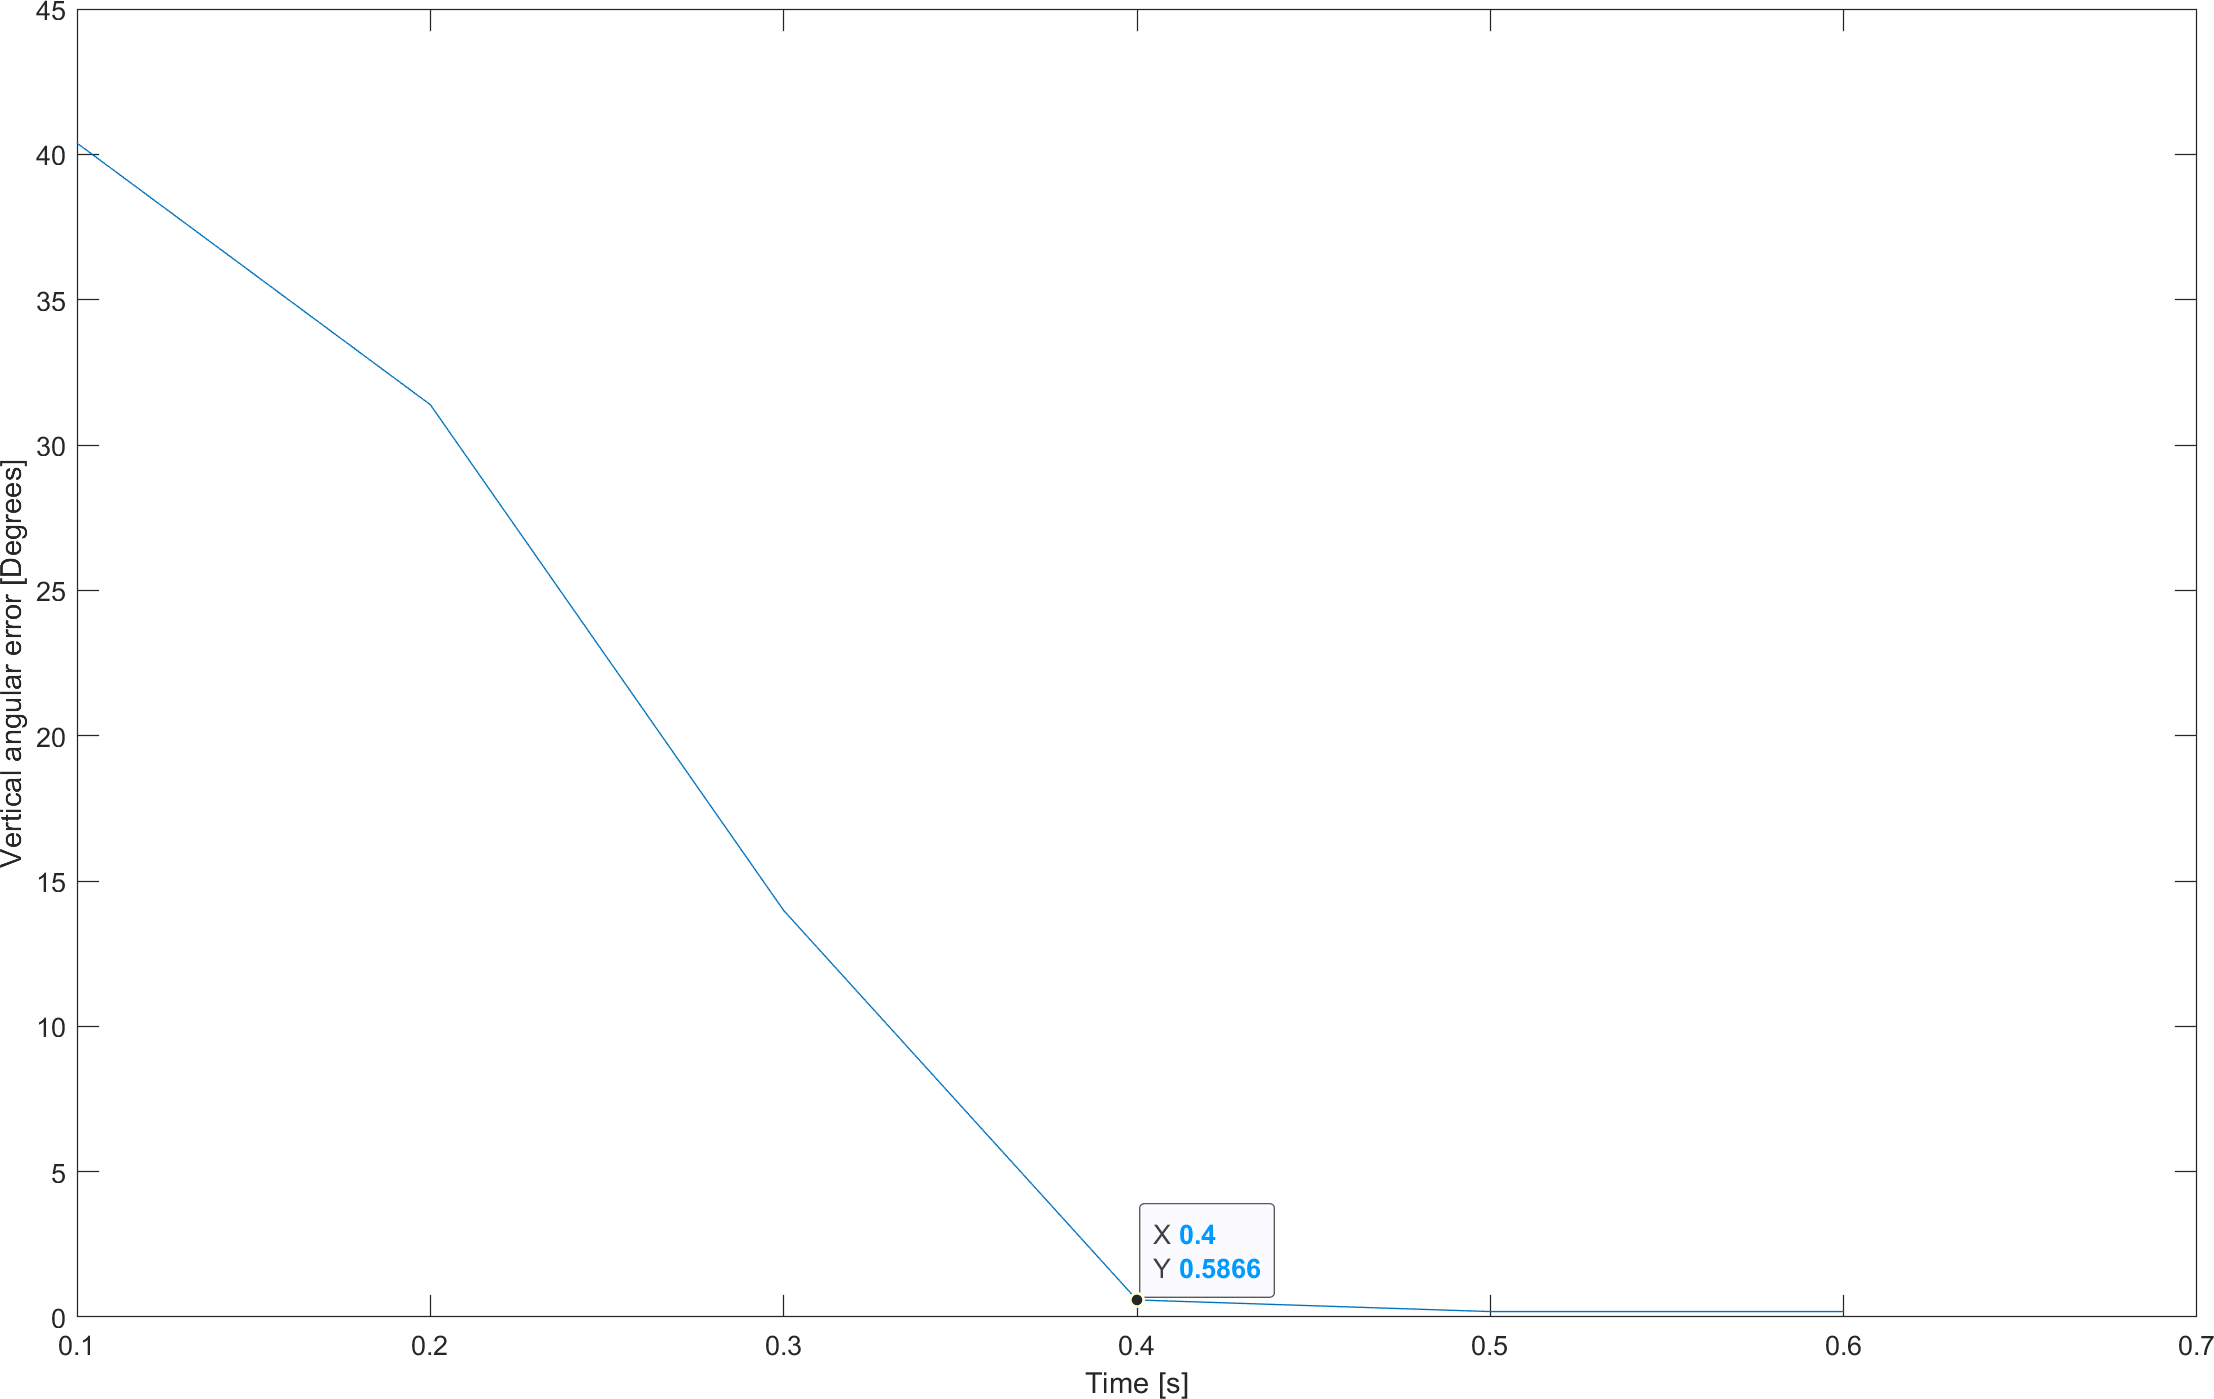
\includegraphics[width = 13 cm]{Vertical_P_controller.png}
\caption{Evolution of vertical angular error from \(40^{\circ}\) step with P-controller}
\label{vert_P}
\end{figure}
Both rise time and settling time of the vertical P controller is 0.4 seconds.
\begin{figure}[H]
\centering
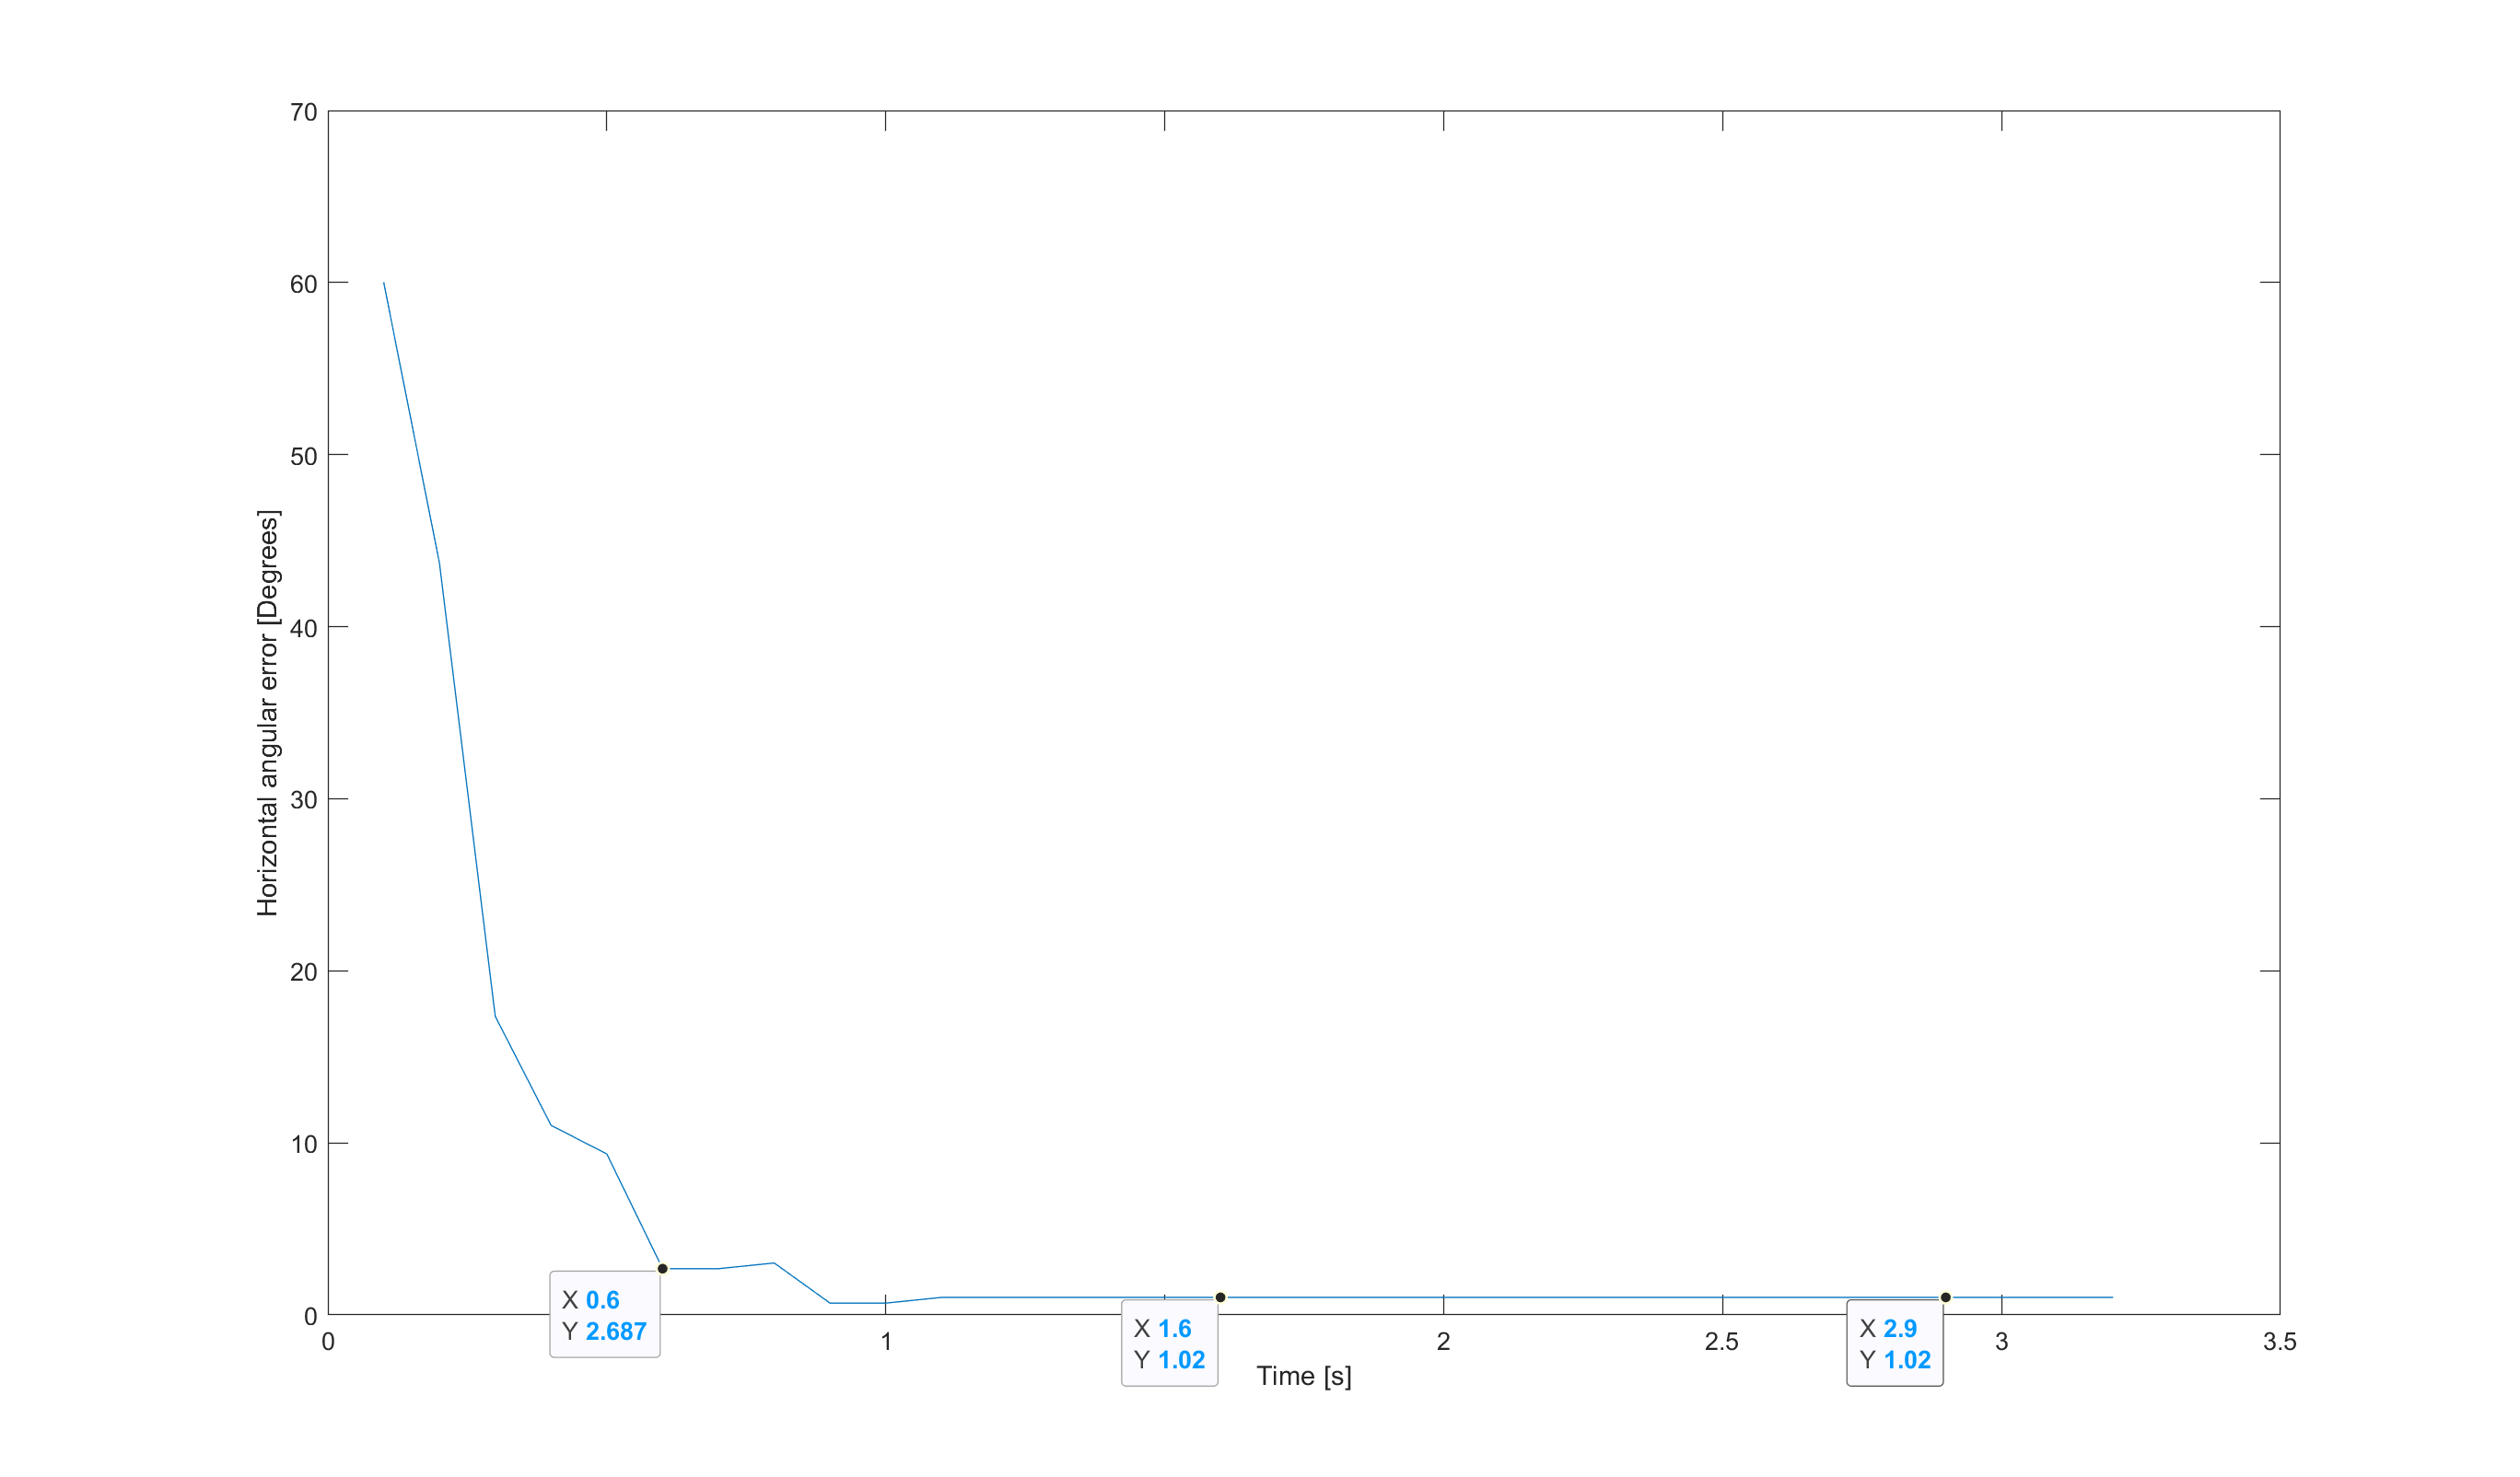
\includegraphics[width = 13 cm]{Horizontal_P_controller.png}
\caption{Evolution of horizontal angular error from \(60^{\circ}\) step with P-controller}
\label{vert_P}
\end{figure}
Rise time of horizontal P controller is 0.6 seconds and settling time is 1.6 seconds

\subsubsection{PI controller}
\begin{figure}[H]
\centering
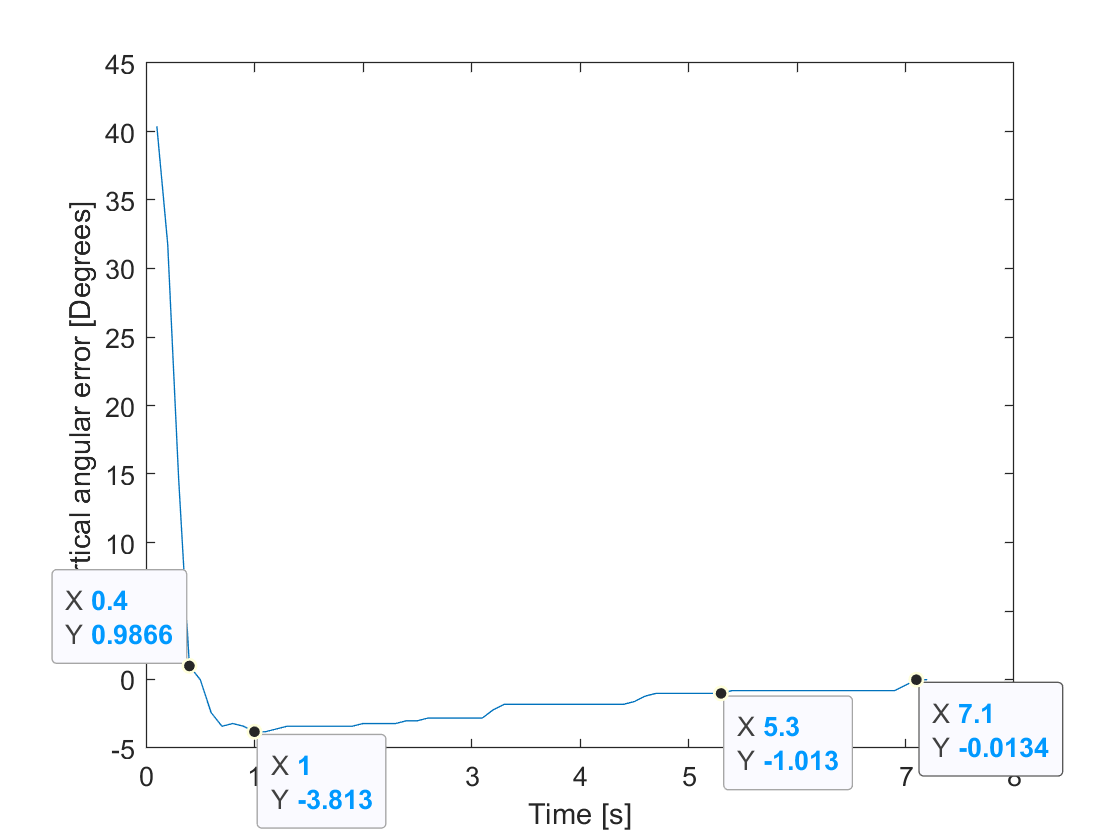
\includegraphics[width = 13 cm]{Vertical_PI_controller.png}
\caption{Evolution of vertical angular error from \(40^{\circ}\) step with P-controller}
\label{vert_P}
\end{figure}
The rise time of the vertical PI controller is 0.4 seconds and the settling time is 7.1 seconds.
\begin{figure}[H]
\centering
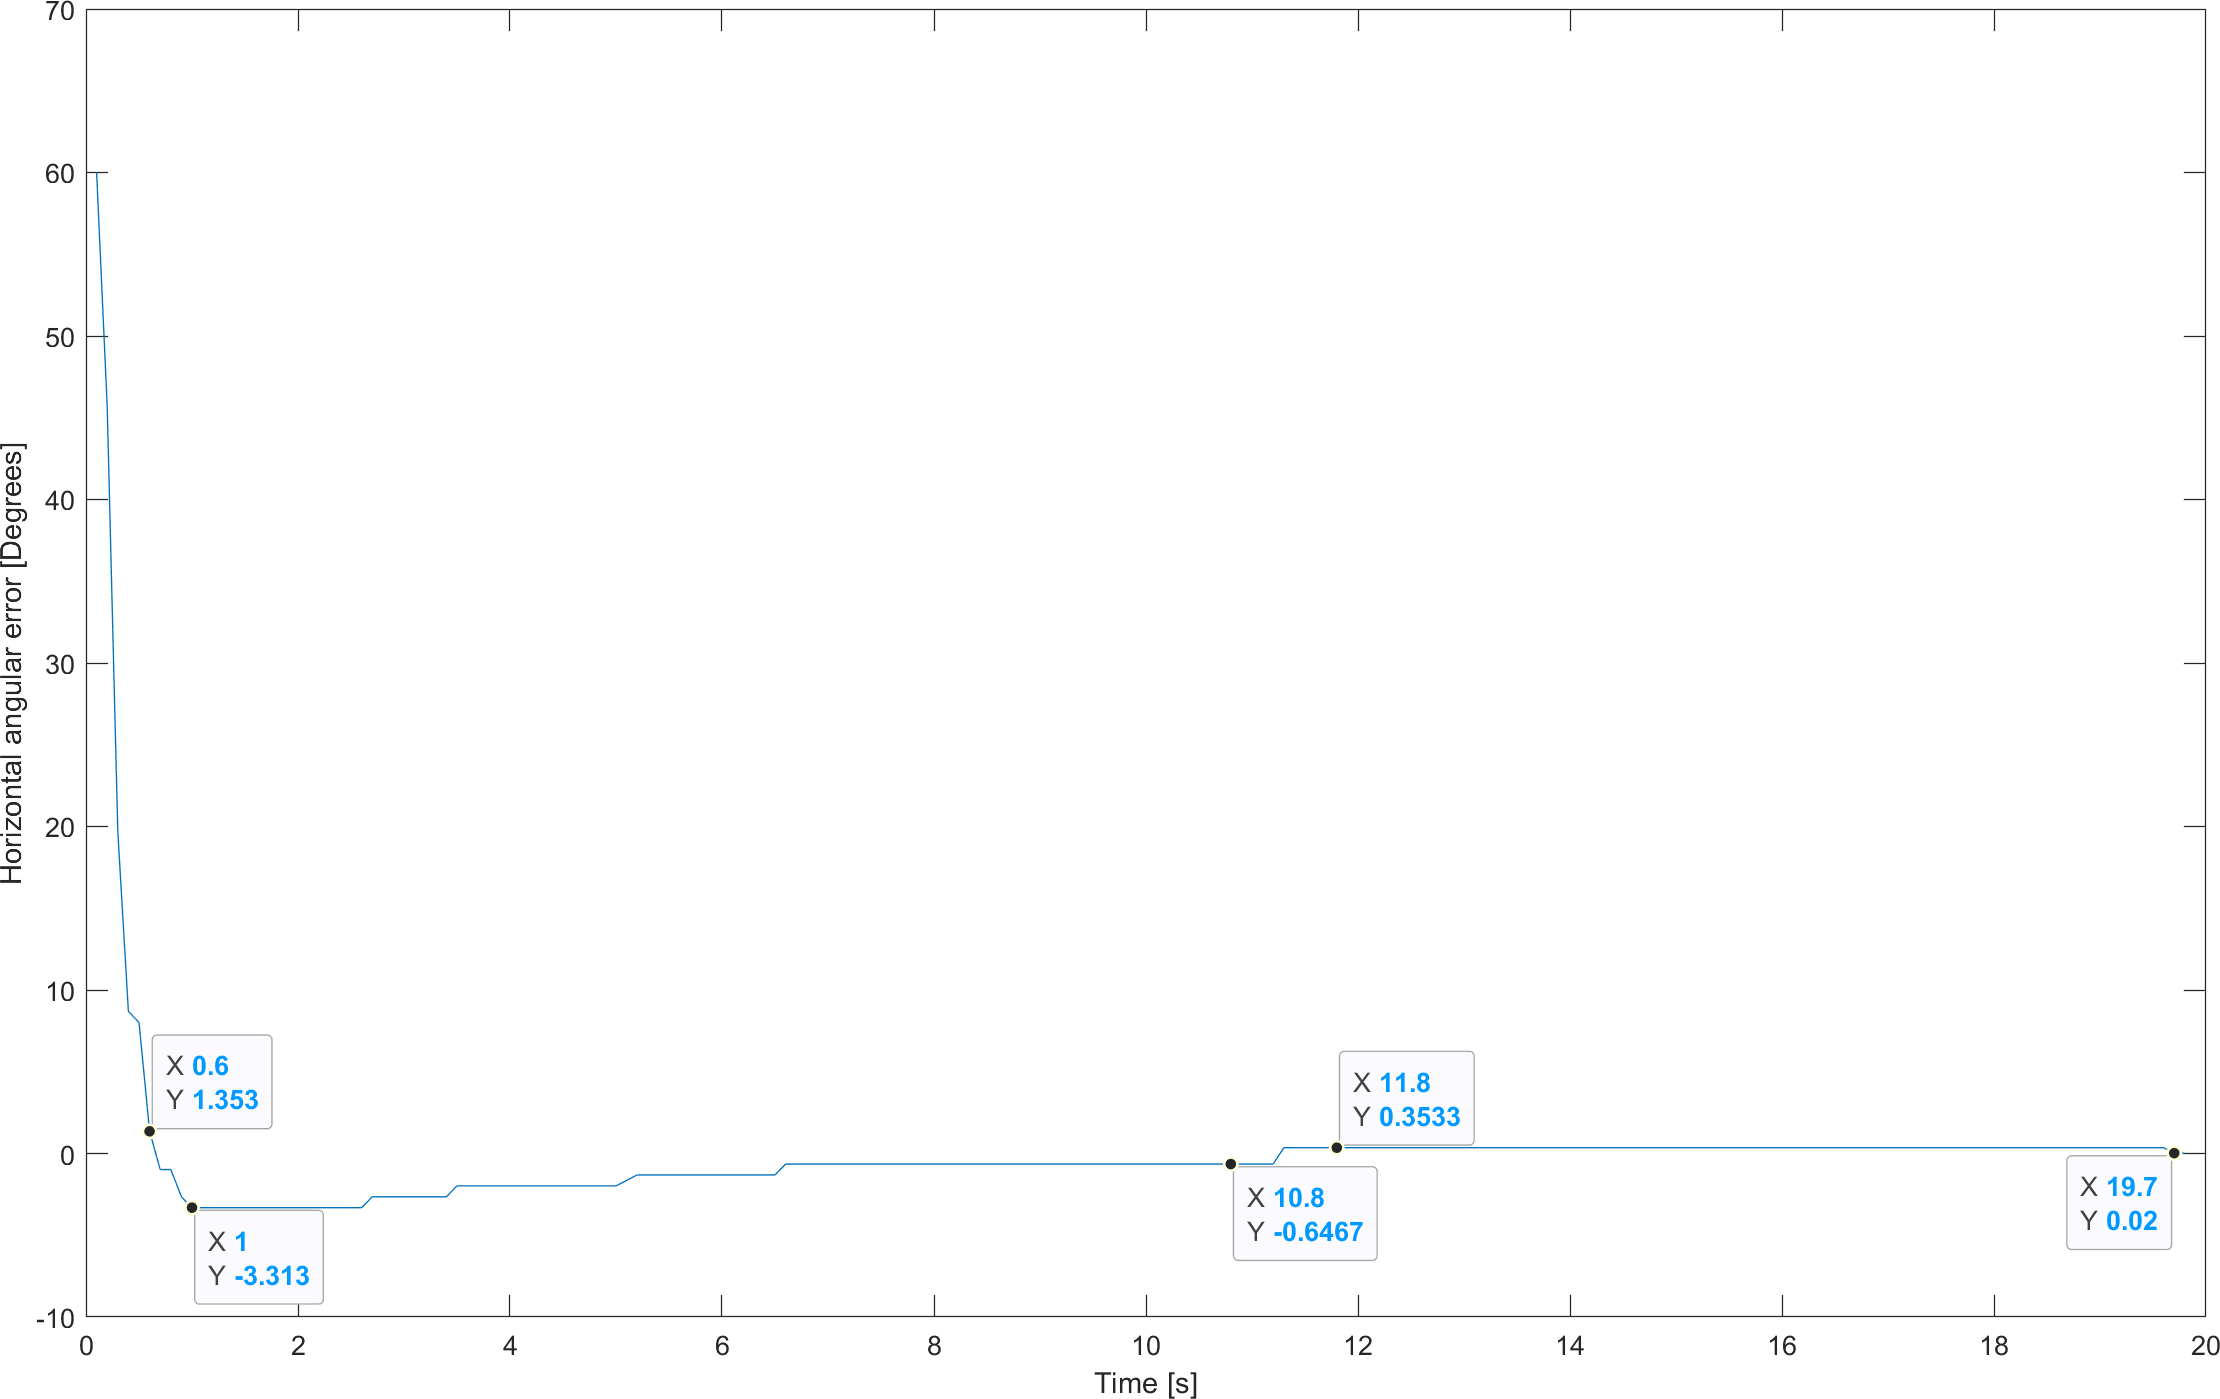
\includegraphics[width = 13 cm]{Horizontal_PI_controller.png}
\caption{Evolution of horizontal angular error from \(60^{\circ}\) step with P-controller}
\label{vert_P}
\end{figure}
Rise time of horizontal PI controller is 0.6 seconds and settling time is 10.8 seconds

\subsubsection{PD controller}
\begin{figure}[H]
\centering
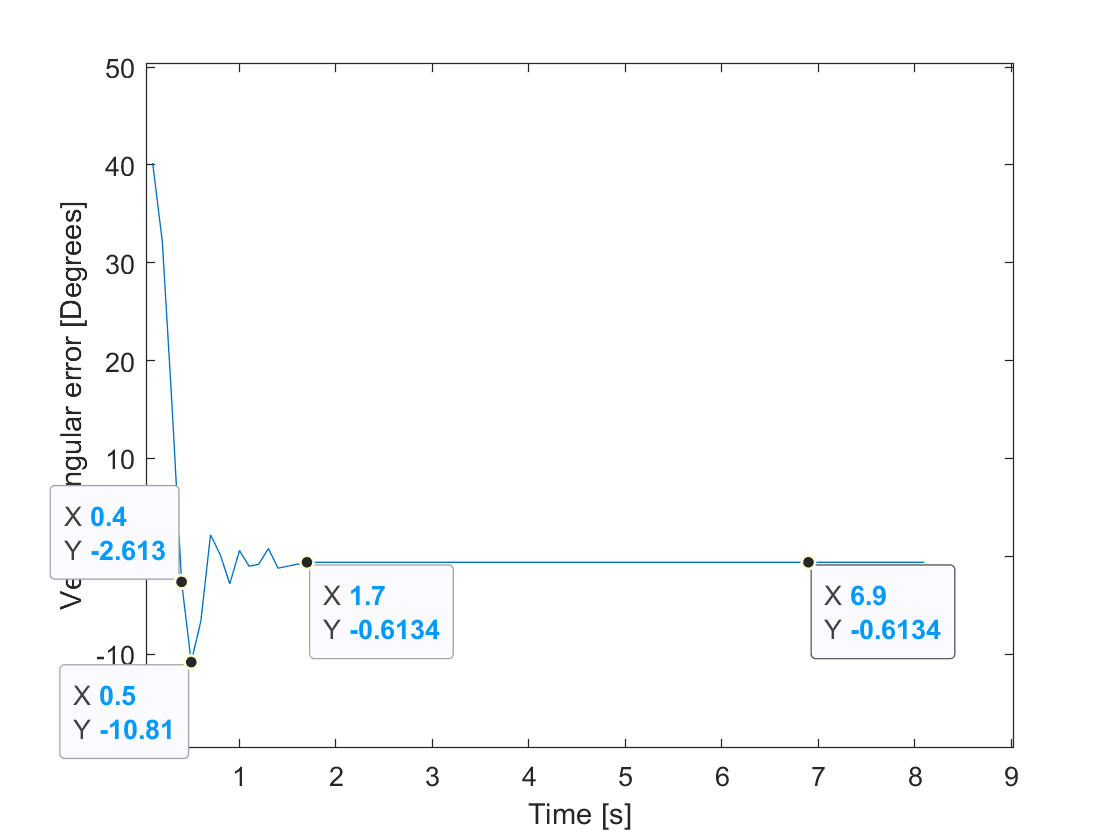
\includegraphics[width = 13 cm]{Vertical_PD_controller.png}
\caption{Evolution of vertical angular error from \(40^{\circ}\) step with P-controller}
\label{vert_P}
\end{figure}
The rise time of the vertical PD controller is 0.4 seconds and the settling time is 1.7 seconds.
\begin{figure}[H]
\centering
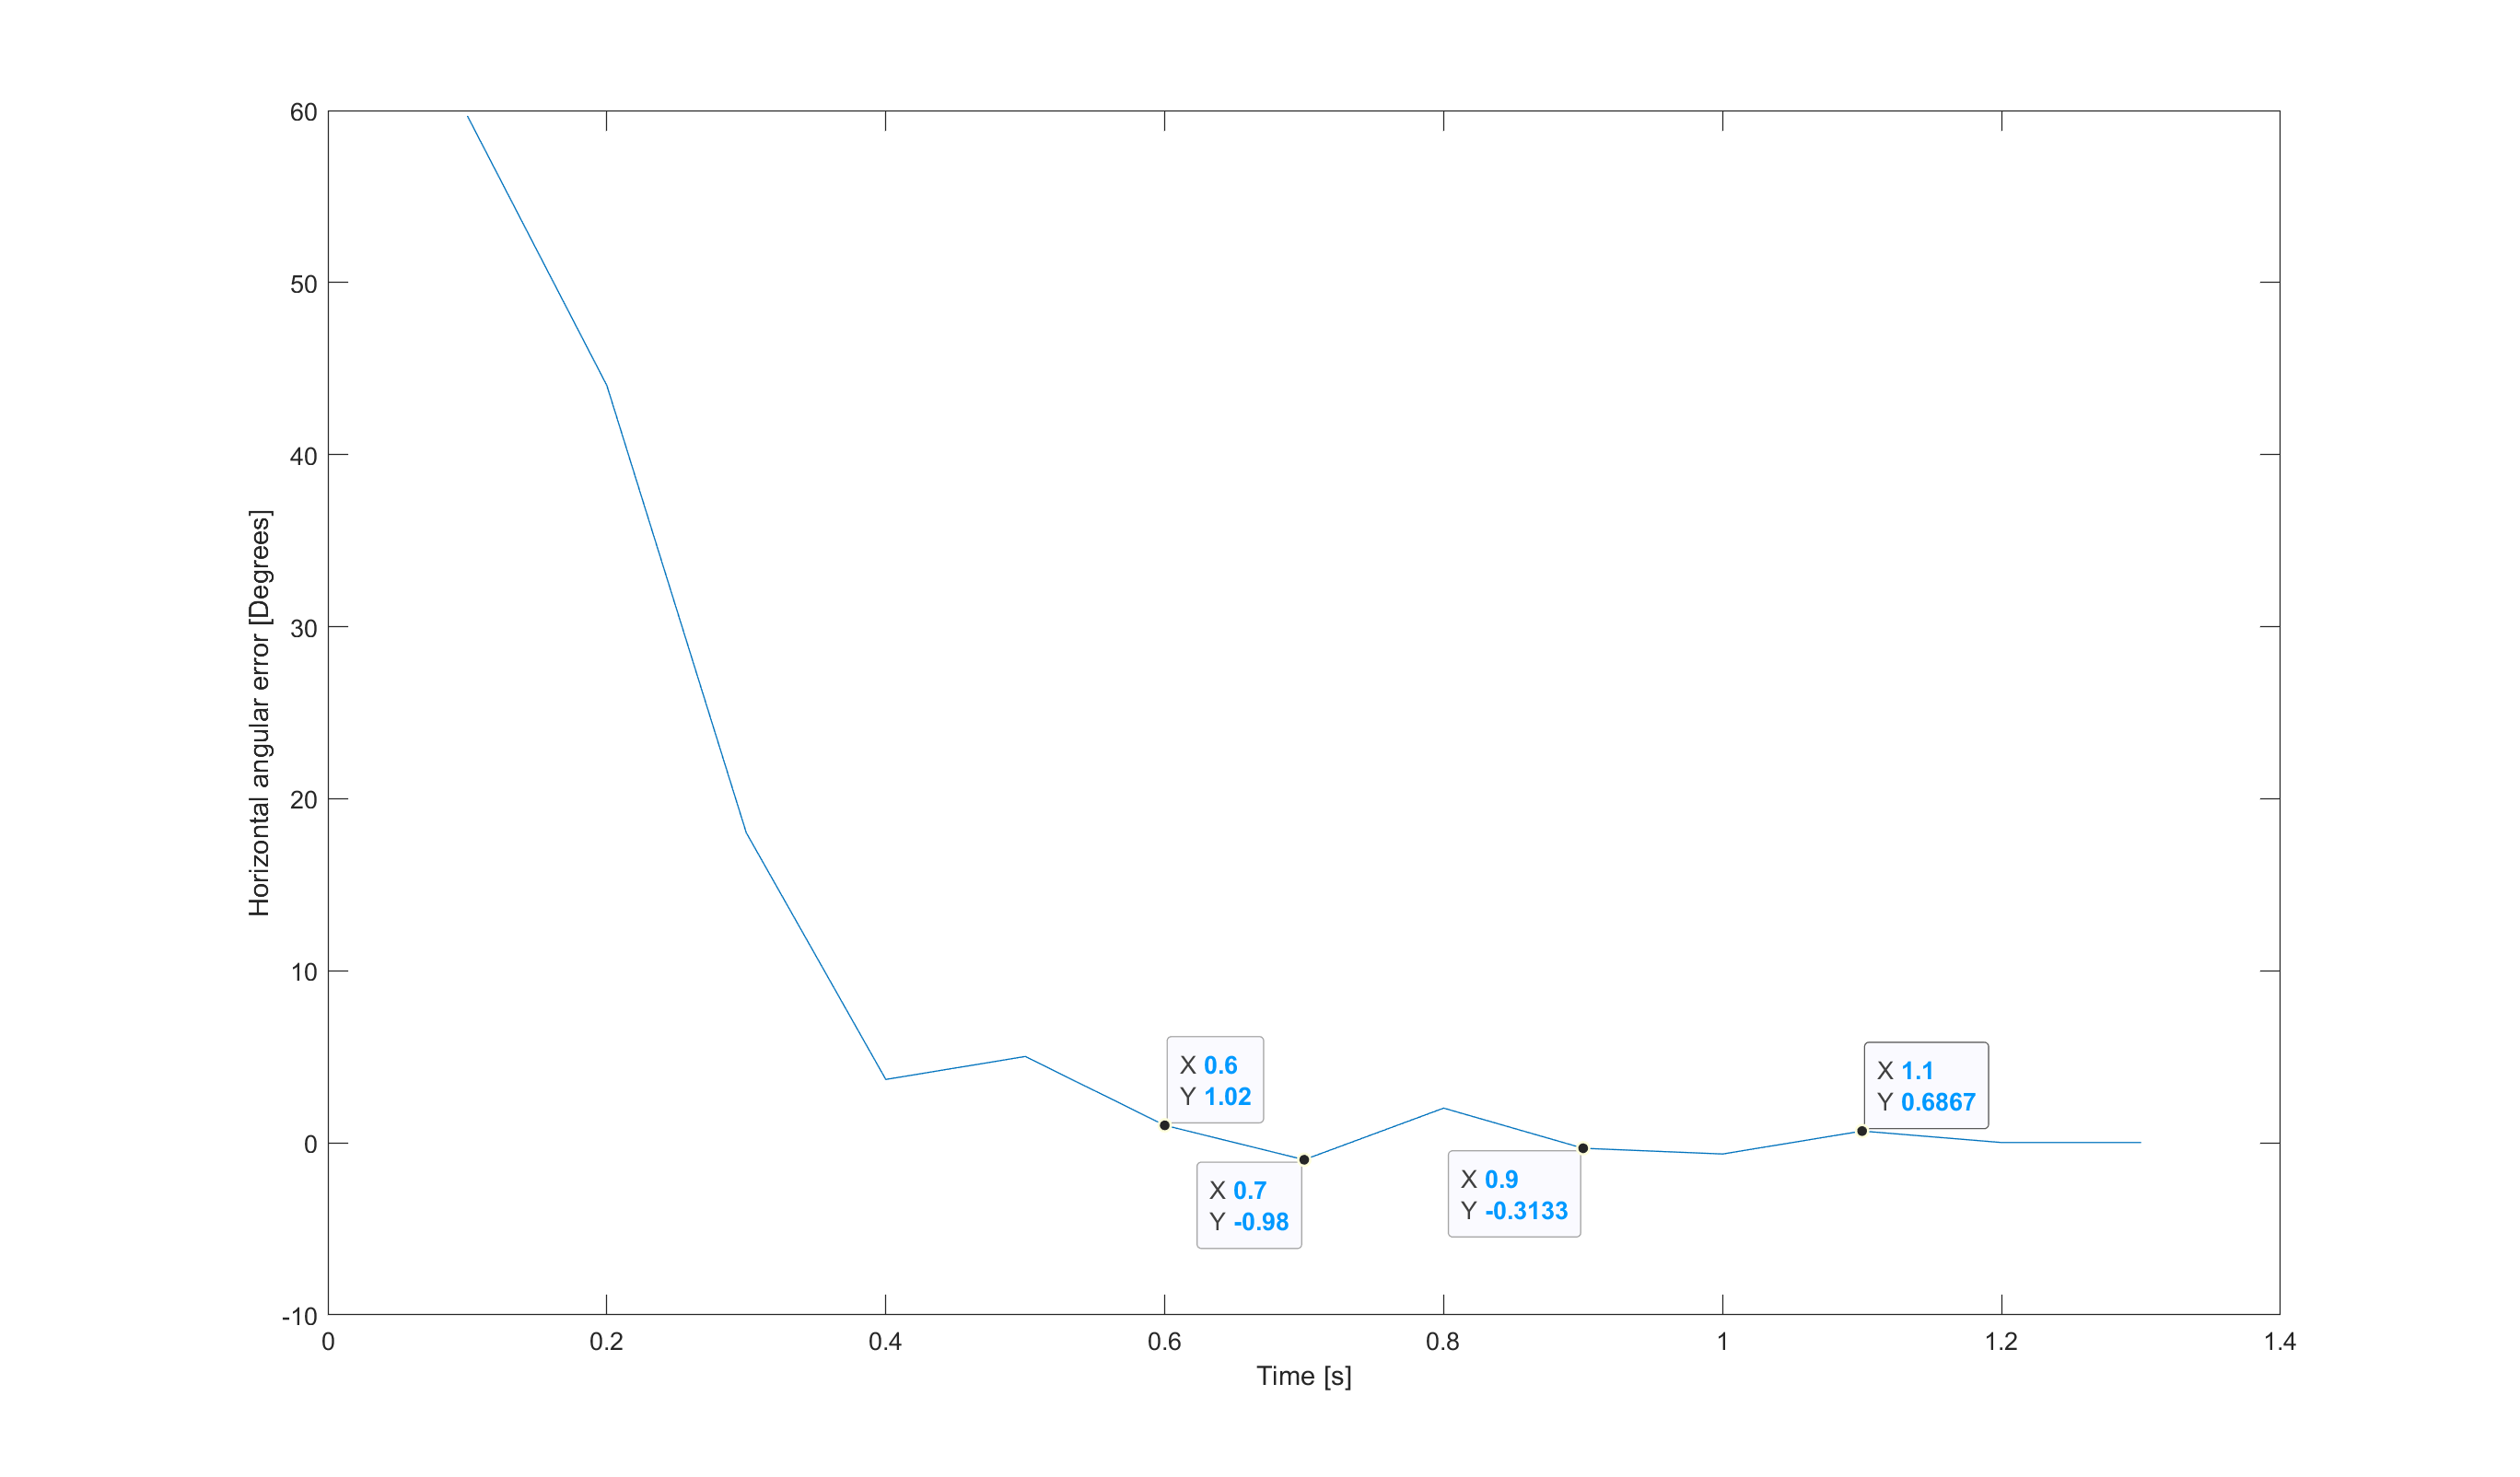
\includegraphics[width = 13 cm]{Horizontal_PD_controller.png}
\caption{Evolution of horizontal angular error from \(60^{\circ}\) step with P-controller}
\label{vert_P}
\end{figure}
Rise time of horizontal PI controller is 0.6 seconds and settling time is 0.9 seconds

\subsubsection{PID controller}
\begin{figure}[H]
\centering
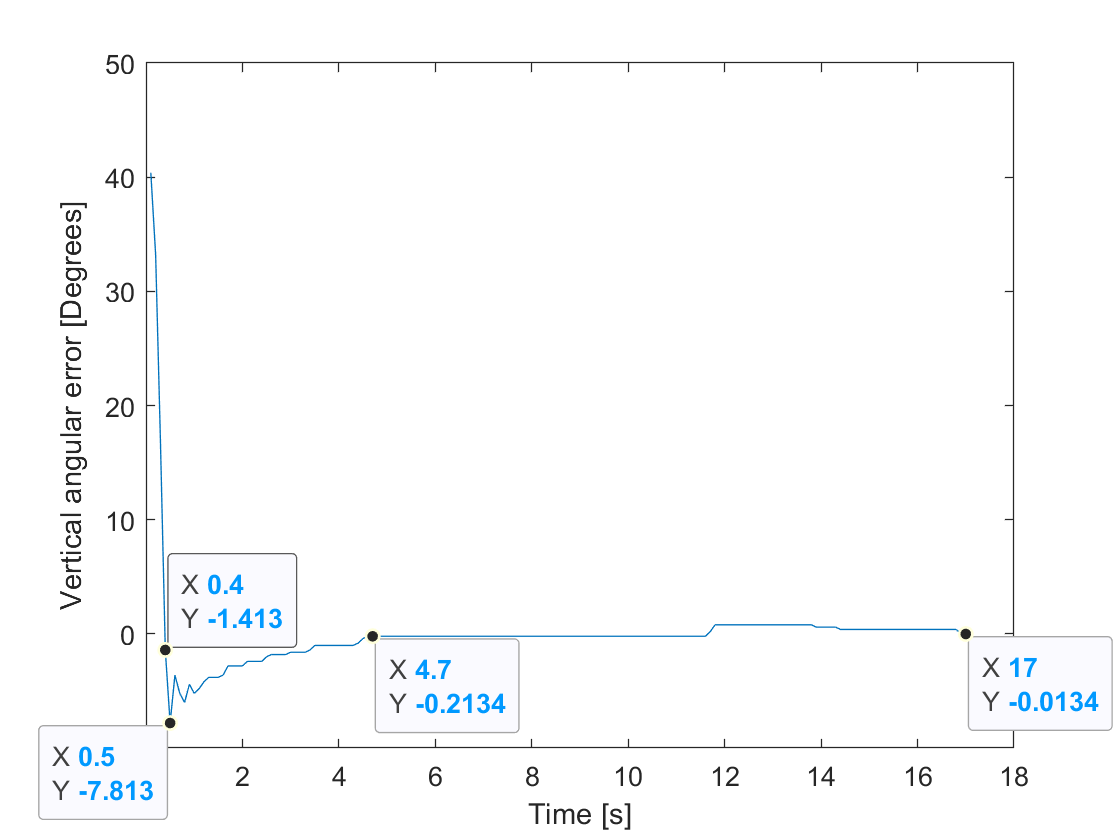
\includegraphics[width = 13 cm]{Vertical_PID_controller.png}
\caption{Evolution of vertical angular error from \(40^{\circ}\) step with P-controller}
\label{vert_P}
\end{figure}
The rise time of the vertical PD controller is between 0.4 and 0.5 seconds and the settling time is 4.7 seconds.
\begin{figure}[H]
\centering
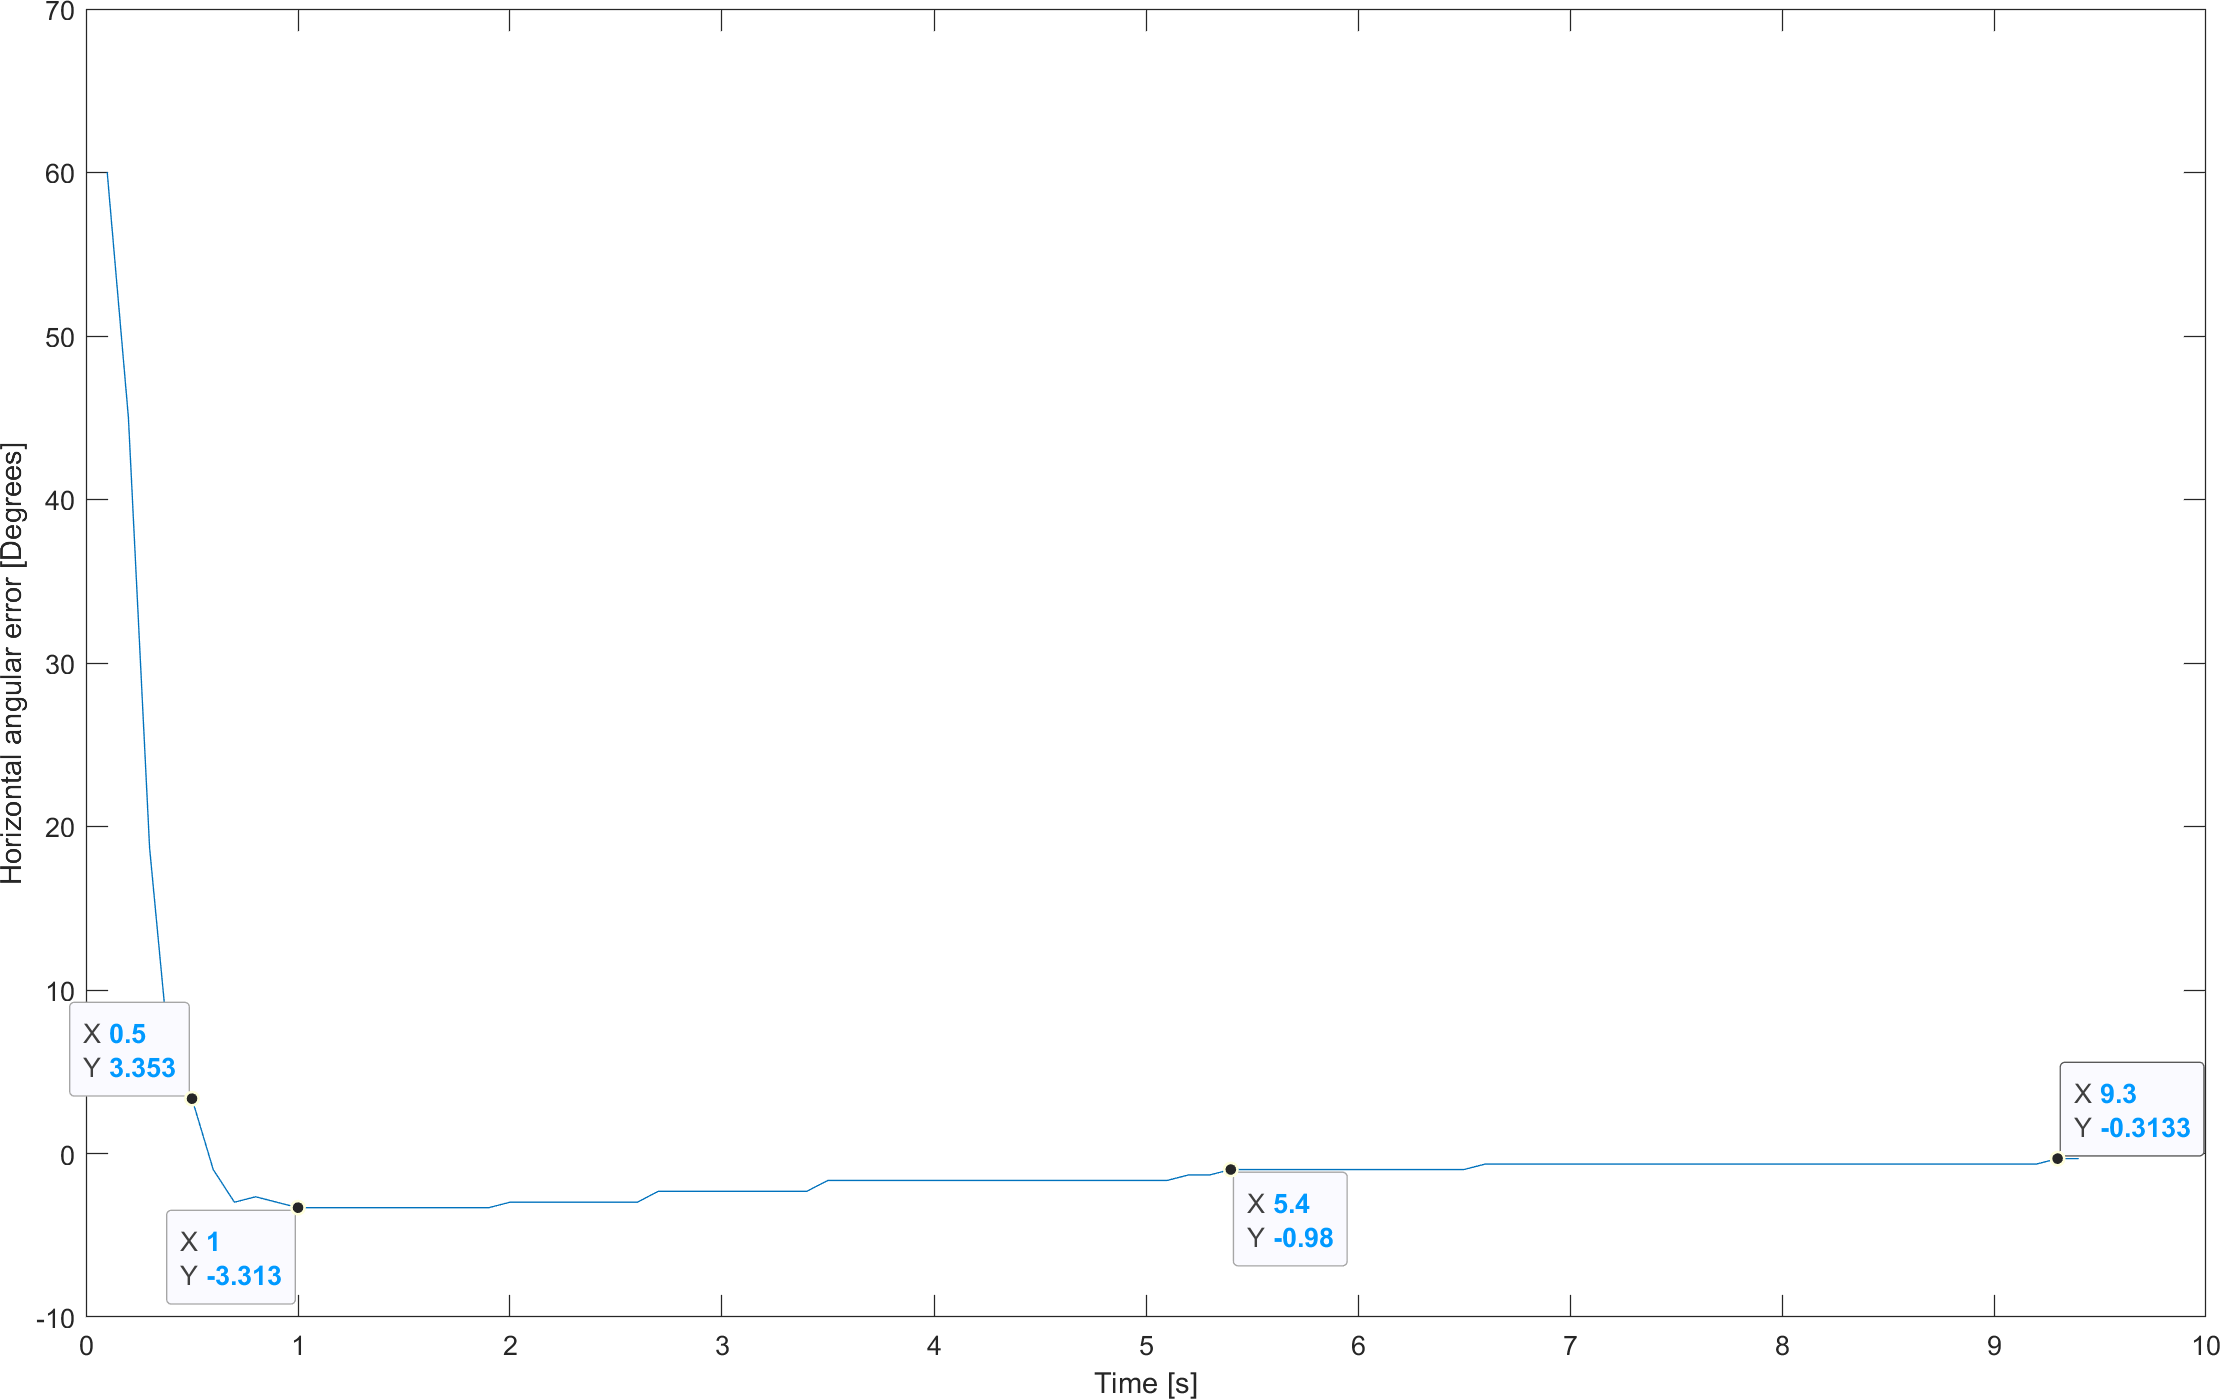
\includegraphics[width = 13 cm]{Horizontal_PID_controller.png}
\caption{Evolution of horizontal angular error from \(60^{\circ}\) step with P-controller}
\label{vert_P}
\end{figure}
Rise time of horizontal PI controller is between 0.5 and 0.6 seconds and settling time is 5.4 seconds

\subsubsection{BrickPi3 library for controlling robot arm movement}
\begin{figure}[H]
\centering
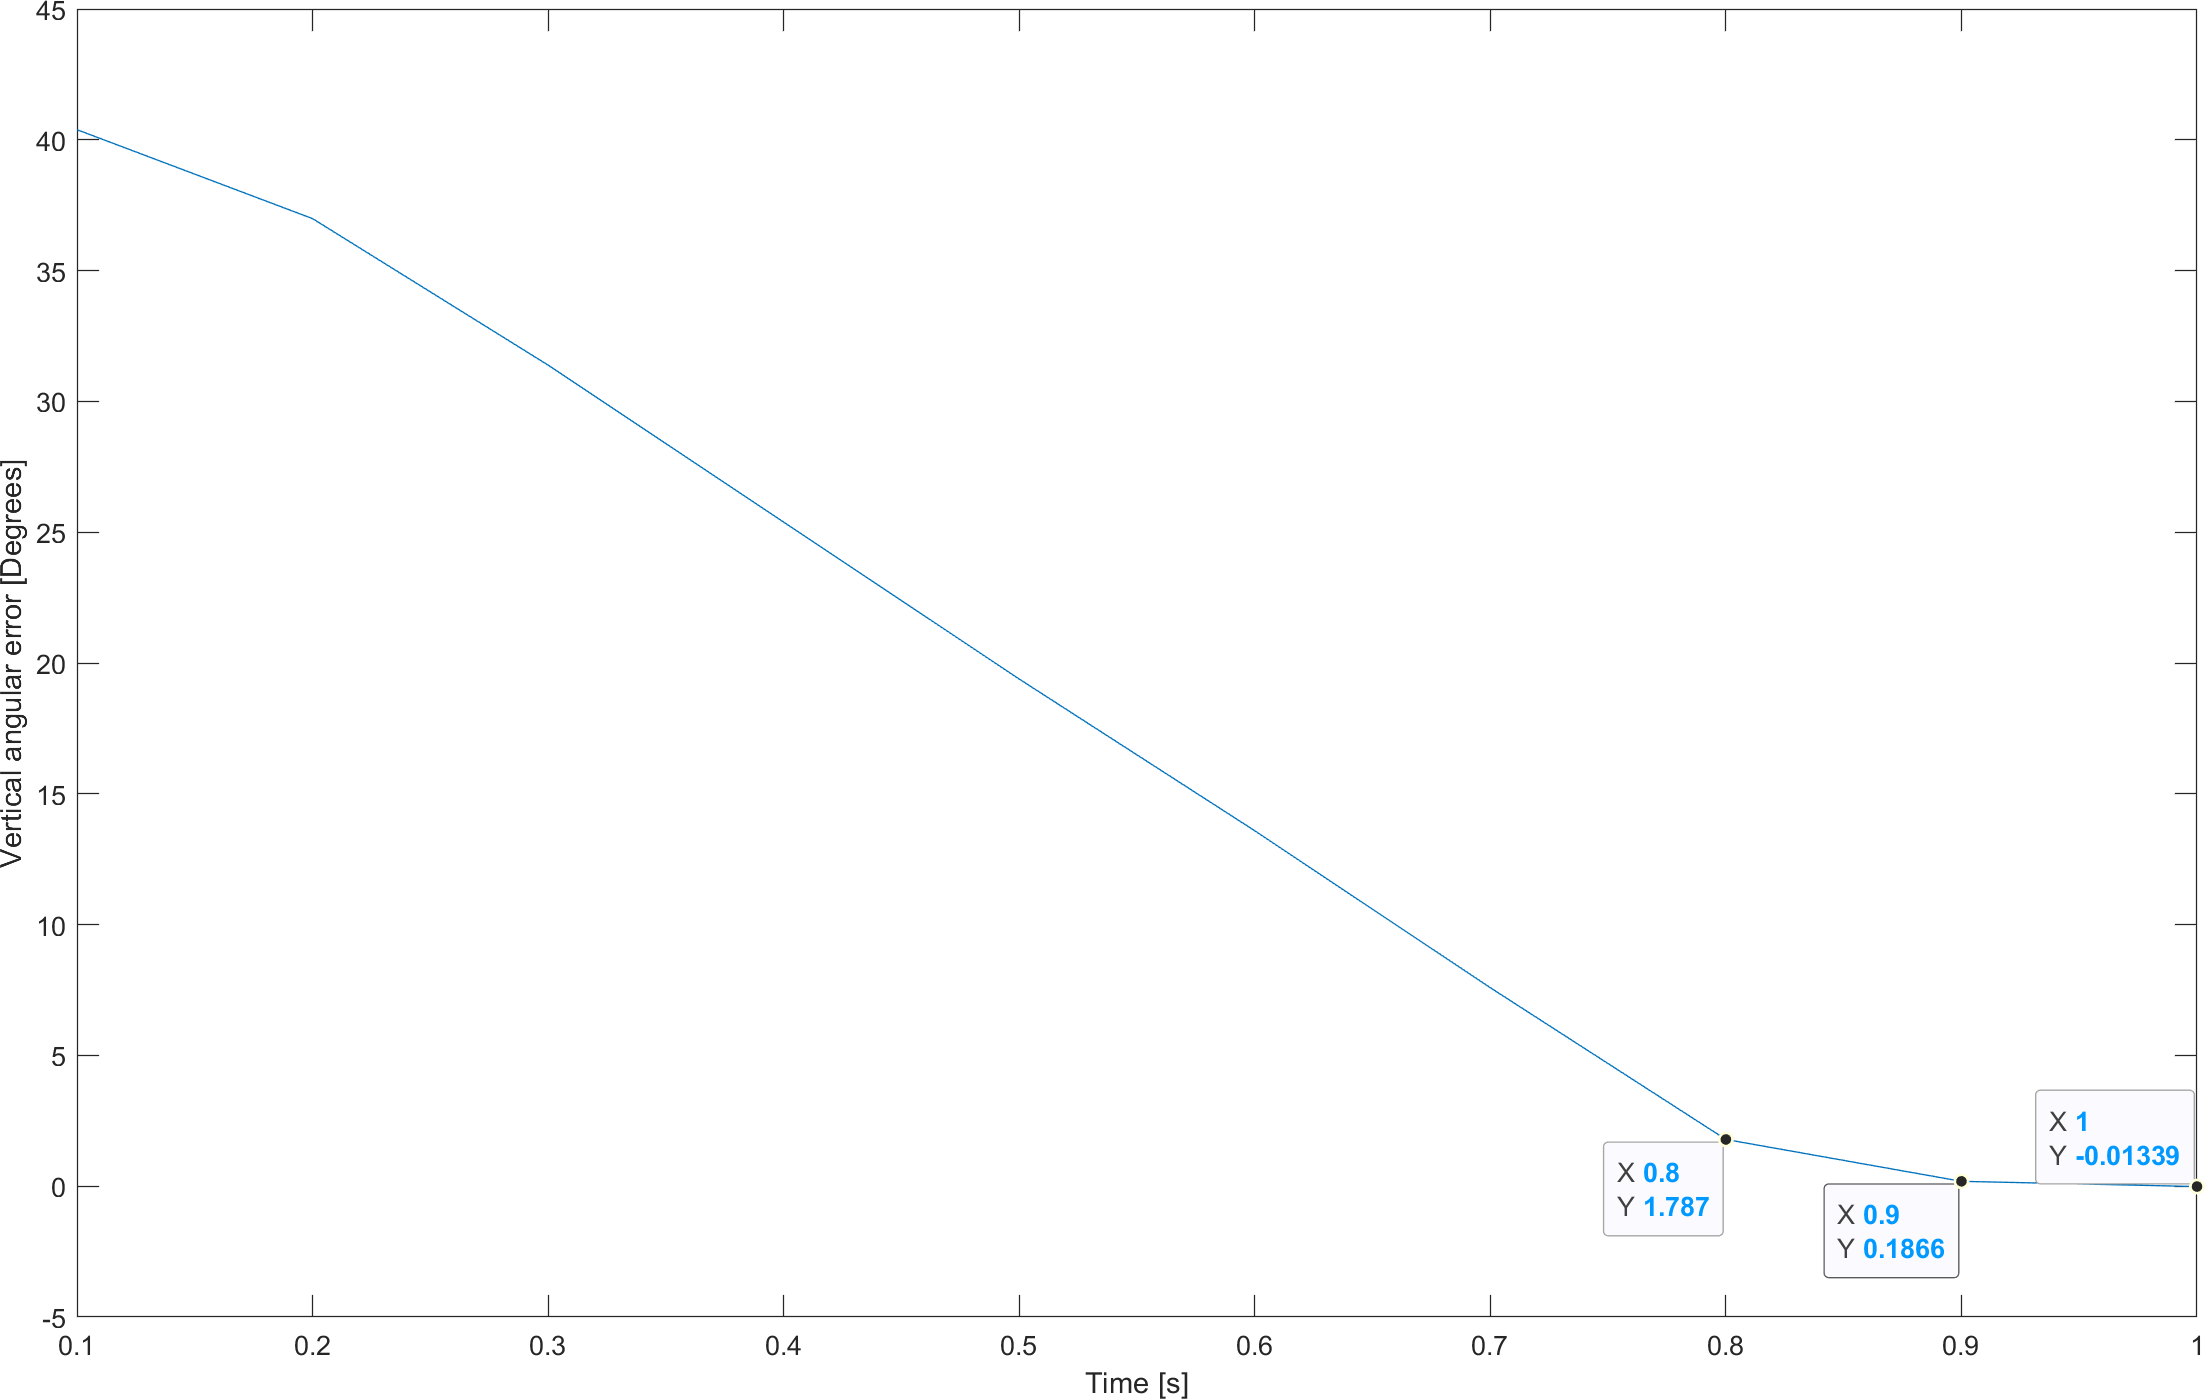
\includegraphics[width = 13 cm]{Vertical_built_in_functions.png}
\caption{Evolution of vertical angular error from \(40^{\circ}\) step with P-controller}
\label{vert_P}
\end{figure}
The rise time of the vertical PD controller is between 0.8 seconds and the settling time is 0.9 seconds.
\begin{figure}[H]
\centering
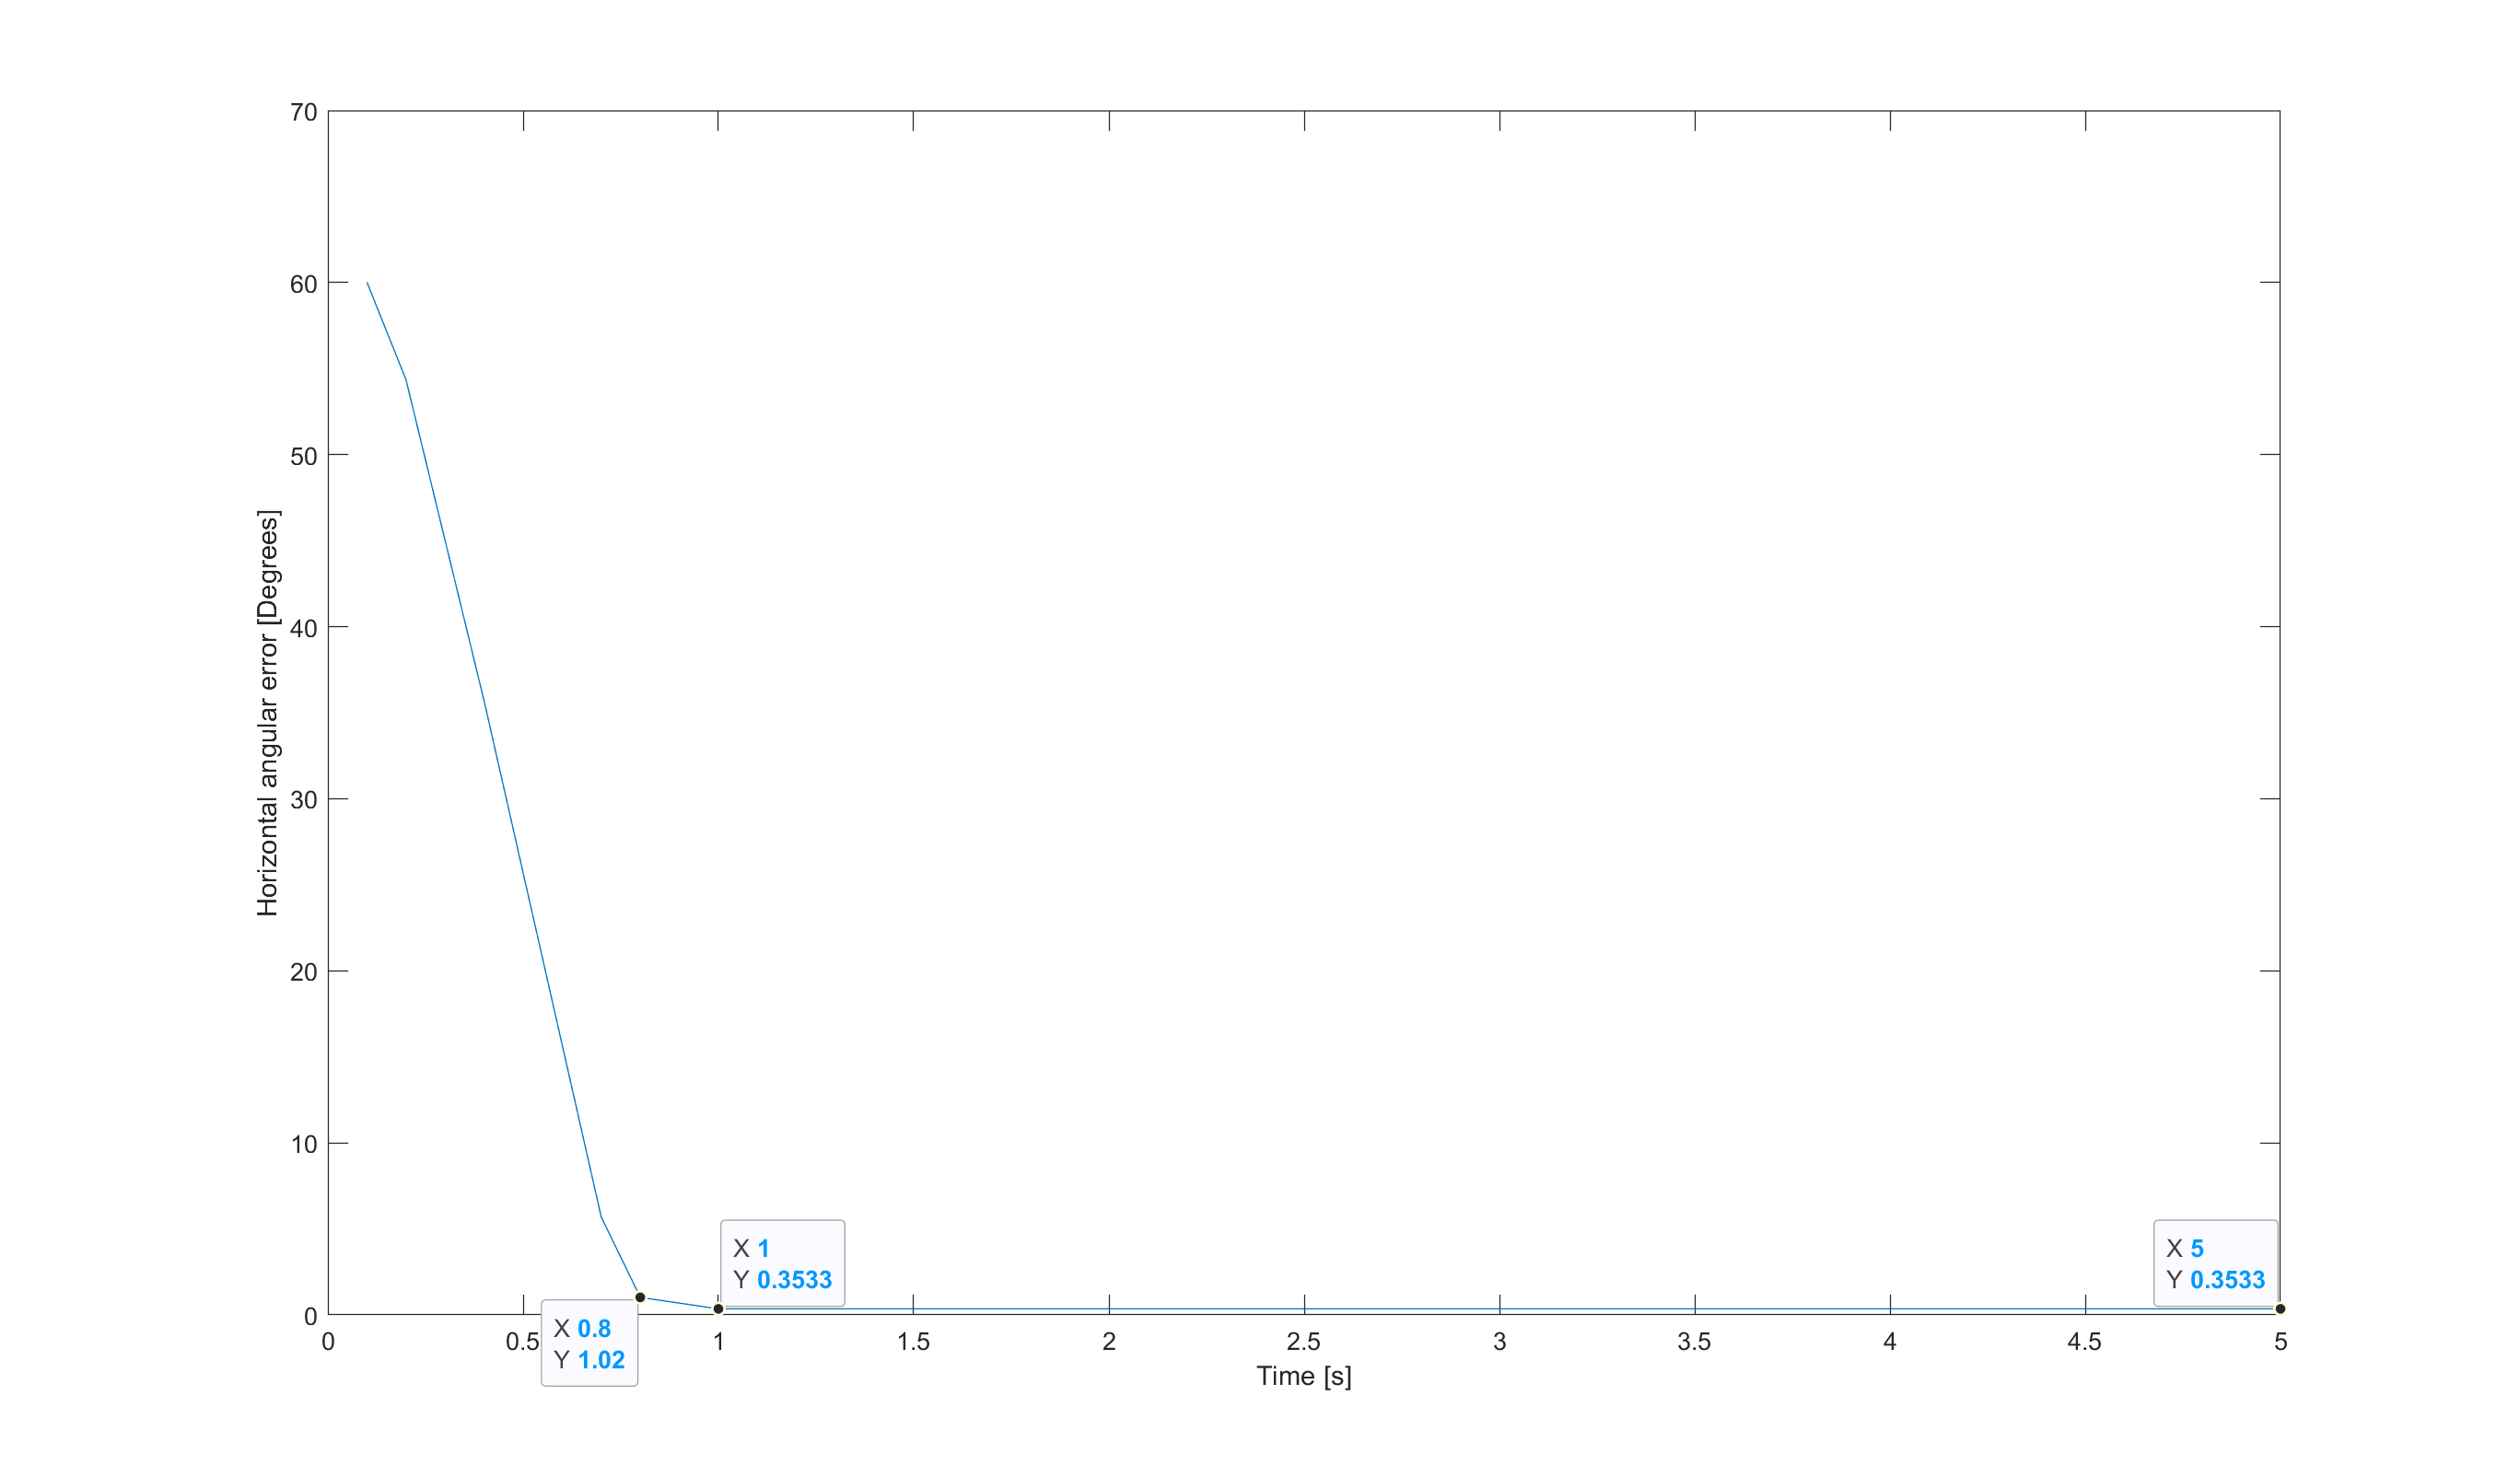
\includegraphics[width = 13 cm]{Horizontal_built_in_funtion.png}
\caption{Evolution of horizontal angular error from \(60^{\circ}\) step with P-controller}
\label{vert_P}
\end{figure}
Rise time of horizontal PI controller is between 0.8 seconds and settling time is 1 second

\subsection{Ziegler Nichols tuning results}
The controllers mentioned above was tuned with a Ziegler Nichols approach and two plots of undamped oscillations for vertical and horizontal arm movements are shown in figure \ref{vert_osc} and \ref{Hor_osc}
\begin{figure}[H]
\centering
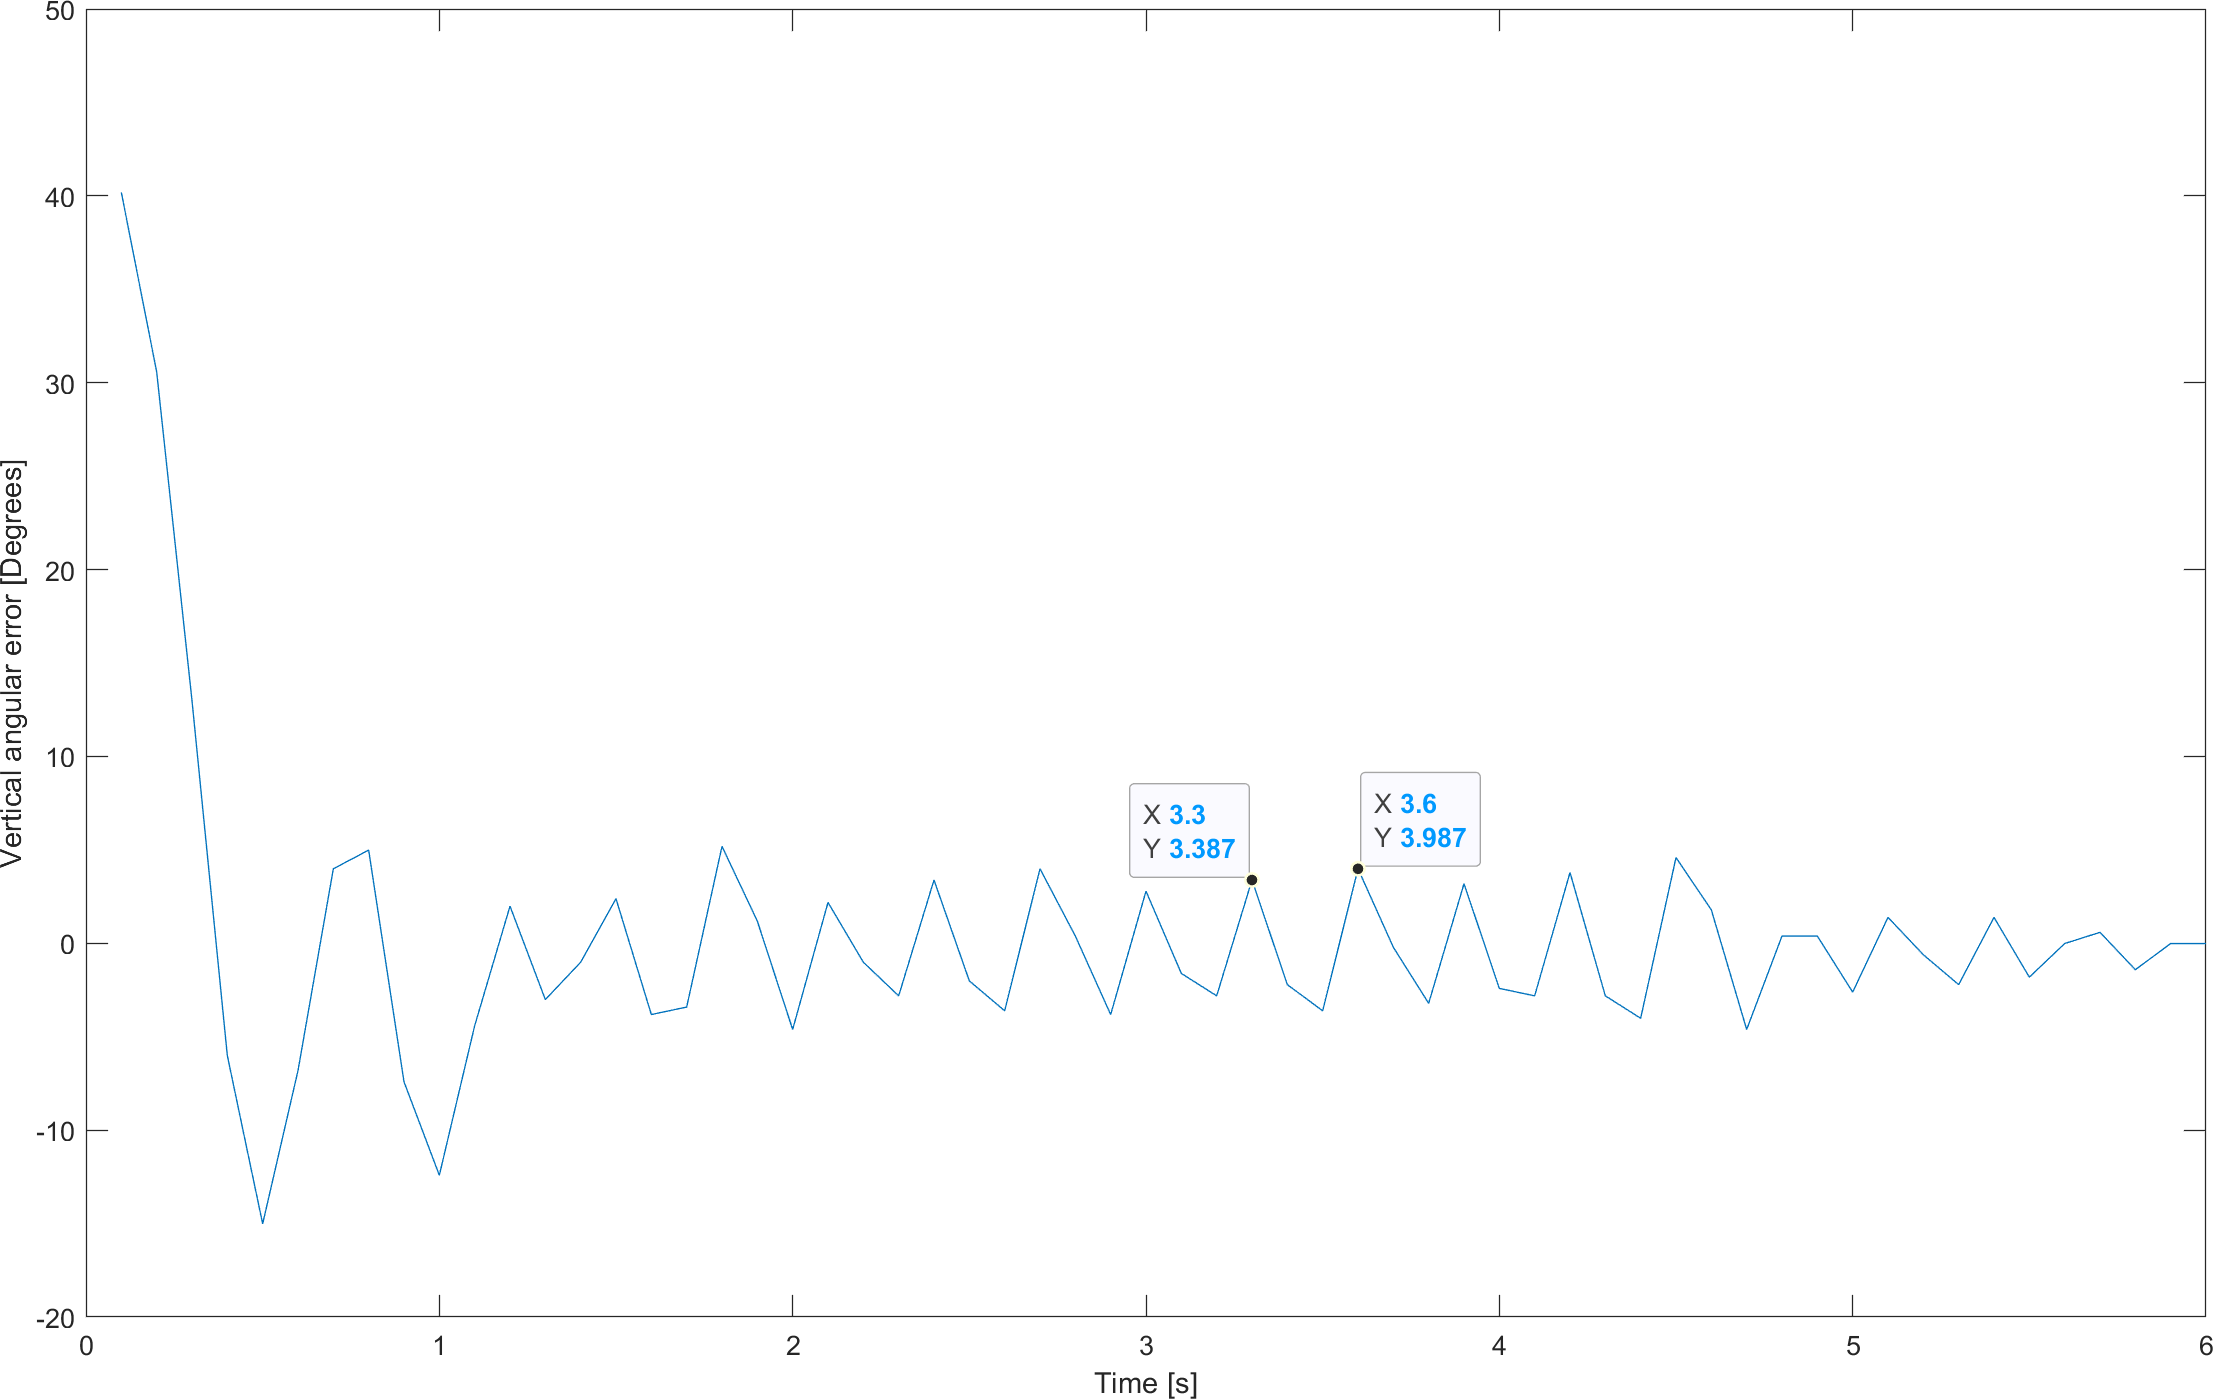
\includegraphics[width = 13 cm]{Vertical_undamped_oscillation.png}
\caption{Evolution of vertical angular error from \(40^{\circ}\) step with P-controller}
\label{vert_osc}
\end{figure}
\begin{figure}[H]
\centering
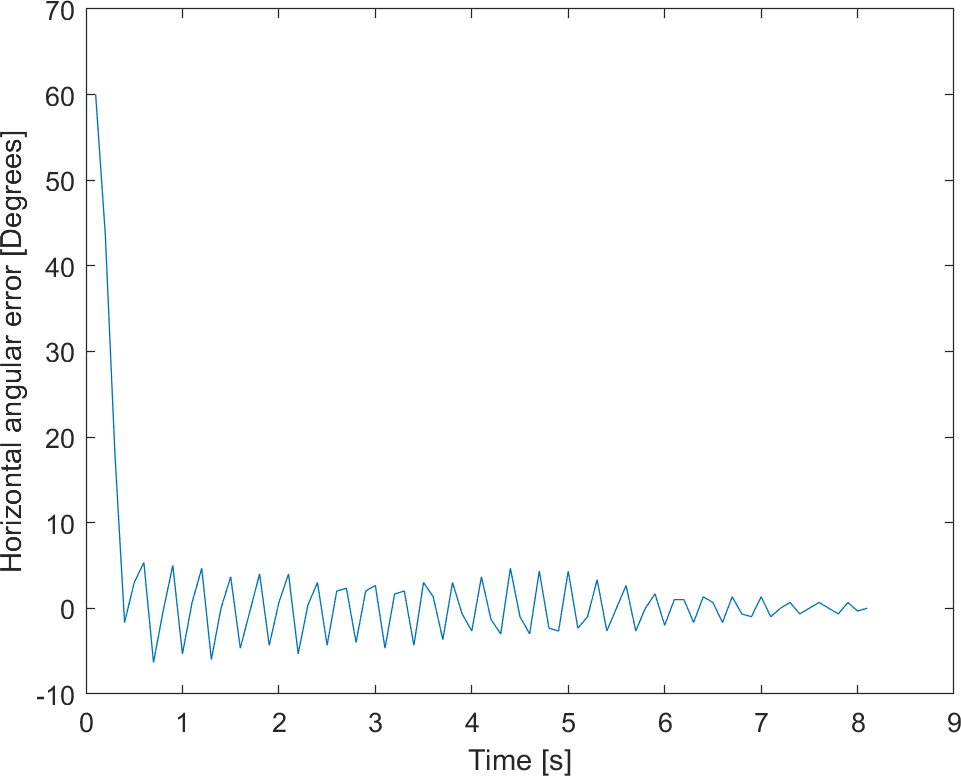
\includegraphics[width = 13 cm]{Horizontal_undamped_oscillation.png}
\caption{Evolution of vertical angular error from \(40^{\circ}\) step with P-controller}
\label{Hor_osc}
\end{figure}
